%%%%%%%%%%%%%%%%%%%%%%%%%%%%%%%%%%%%%%%%%%%%%%%%%%%%%%%%%%%%%%%%%%%%%%%%%%%%%%%%%%%%
%Do not alter this block of commands.  If you're proficient at LaTeX, you may include additional packages, create macros, etc. immediately below this block of commands, but make sure to NOT alter the header, margin, and comment settings here. 
\documentclass[12pt]{article}
 \usepackage[margin=1in]{geometry} 
\usepackage{amsmath,amsthm,amssymb,amsfonts, enumitem, fancyhdr, color, hyperref,comment, graphicx, environ,mathtools, bbm, tikz, setspace, cleveref,listings, dcolumn}
\usepackage{array, multirow, caption, booktabs}
\usepackage{ mathrsfs }
\captionsetup[table]{name=Table}
\renewcommand{\thetable}{\Roman{table}}
\usetikzlibrary{matrix,positioning}
\tikzset{bullet/.style={circle,draw=black,inner sep=8pt}}
\DeclareMathOperator*{\argmax}{arg\,max}
\DeclareMathOperator*{\argmin}{arg\,min}
\DeclareMathOperator*{\Var}{\text{Var}}
\DeclareMathOperator*{\Cov}{\text{Cov}}

\DeclarePairedDelimiter\norm{\lVert}{\rVert}%
\newtheorem{theorem}{Theorem}
\newtheorem{lemma}[theorem]{Lemma}
\DeclareMathOperator{\eps}{\varepsilon}

\DeclarePairedDelimiter\abs{\lvert}{\rvert}%
\pagestyle{fancy}
\setlength{\headheight}{65pt}
\newenvironment{problem}[2][Problem]{\begin{trivlist}
\item[\hskip \labelsep {\bfseries #1}\hskip \labelsep {\bfseries #2.}]}{\end{trivlist}}
\newenvironment{sol}
    {\emph{Solution:}
    }
    {
    \qed
    }

\lstdefinestyle{myCustomMatlabStyle}{
    %basicstyle=\ttfamily
  language=Matlab,
  numbers=left,
  stepnumber=1,
  numbersep=10pt,
  tabsize=4,
  showspaces=false,
  showstringspaces=false
}
%%%%%%%%%%%%%%%%%%%%%%%%%%%%%%%%%%%%%%%%%%%%%%%%%%%%%%%%%%%%%%%%%%%%%%%%%%%%%%%%%


\usepackage{xcolor}
 

%%%%%%%%%%%%%%%%%%%%%%%%%%%%%%%%%%%%%%%%%%%%%

\rhead{John Higgins\\Econ 761 \\ 5 December, 2022} 

%%%%%%%%%%%%%%%%%%%%%%%%%%%%%%%%%%%%%%%%%%%%%


%%%%%%%%%%%%%%%%%%%%%%%%%%%%%%%%%%%%%%

\begin{document}

\begin{problem}{1}
\end{problem}
\begin{sol}
    I wrote a program to non-parametrically estimate the distribution of valuations and ran it on the provided data. I used a kernel estimator to obtain the estimates $\hat{G}_{M_i, B_i}$ and $\hat{g}_{M_i, B_i}$ for each bidder. Then, using the fact that $\frac{\hat{G}_{M_i, B_i}}{\hat{g}_{M_i, B_i}}$, the implied valuations can be obtained using the following:
    \[u_i = b_i + \frac{G_{M_i, B_i}(b_i \mid b_i; n)}{g_{M_i, B_i}(b_i \mid b_i; n)}\]
    I then estimate the marginal distribution of valuations for each bidder using kernel estimation on the implied valuations. 
    
    I have plotted the kernel density of each bidder below (on the same graph for comparison):
    \begin{center}
        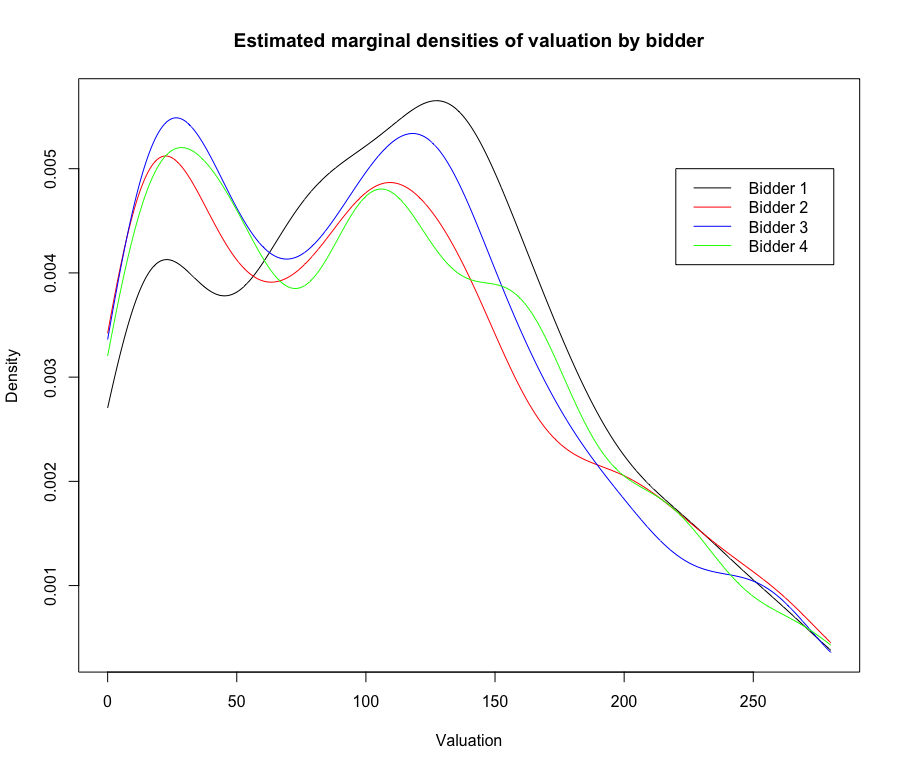
\includegraphics[scale=0.45]{Valuation Dist.png}
    \end{center}
    I have also plotted their bid as a function of their valuation (as well as a 45-degree line). Based on these plots, we can see that bidders are shading their bids (as we would expect in a first price auction).
    \begin{center}
        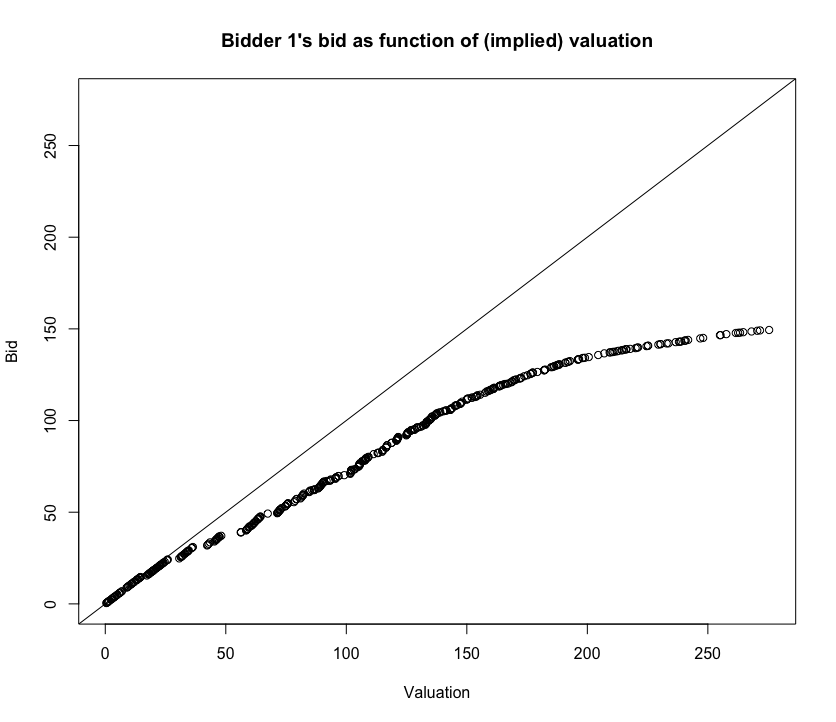
\includegraphics[scale=0.25]{Bid_1.png} 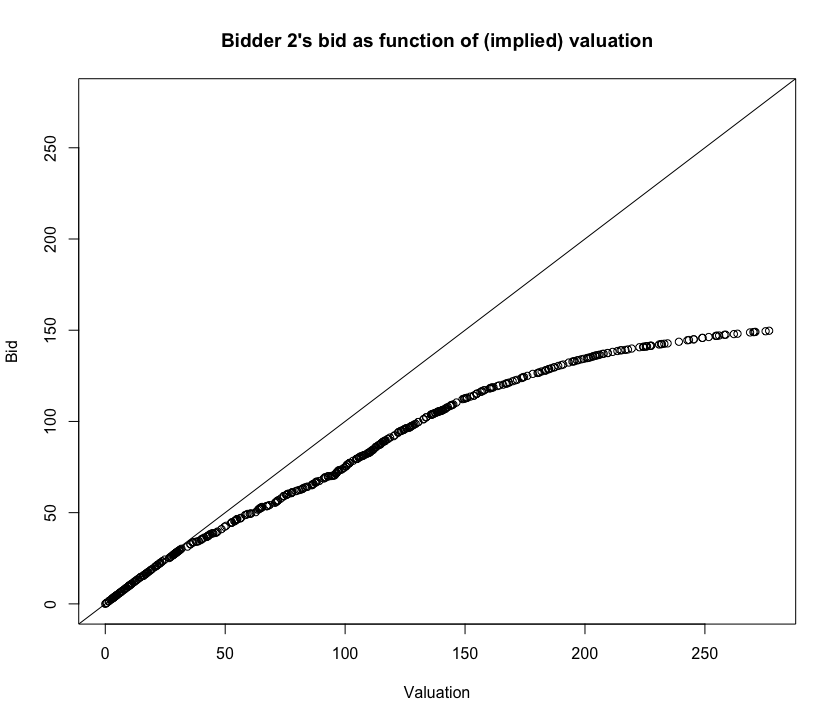
\includegraphics[scale=0.25]{Bid_2.png}\\
        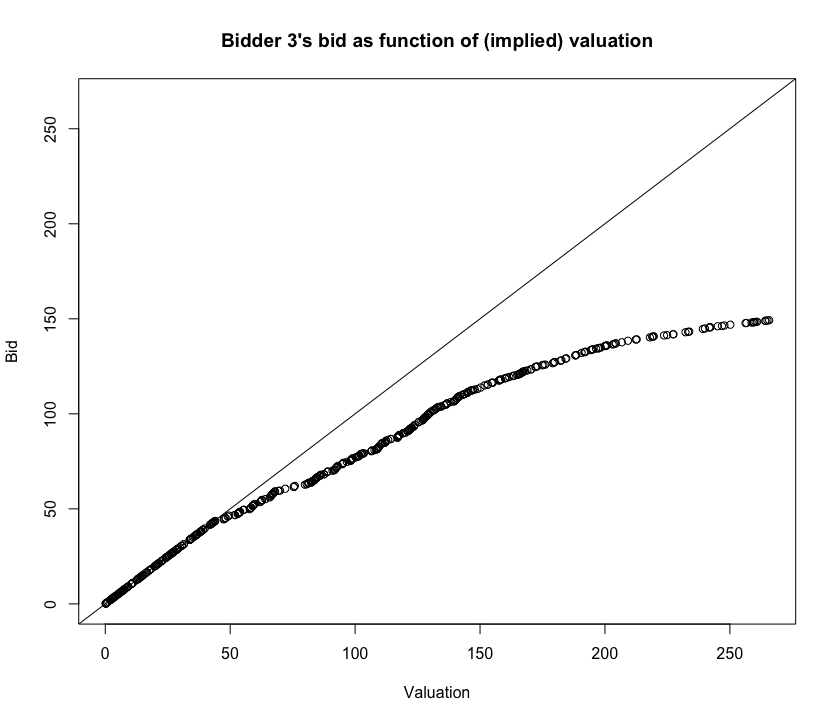
\includegraphics[scale=0.25]{Bid_3.png} 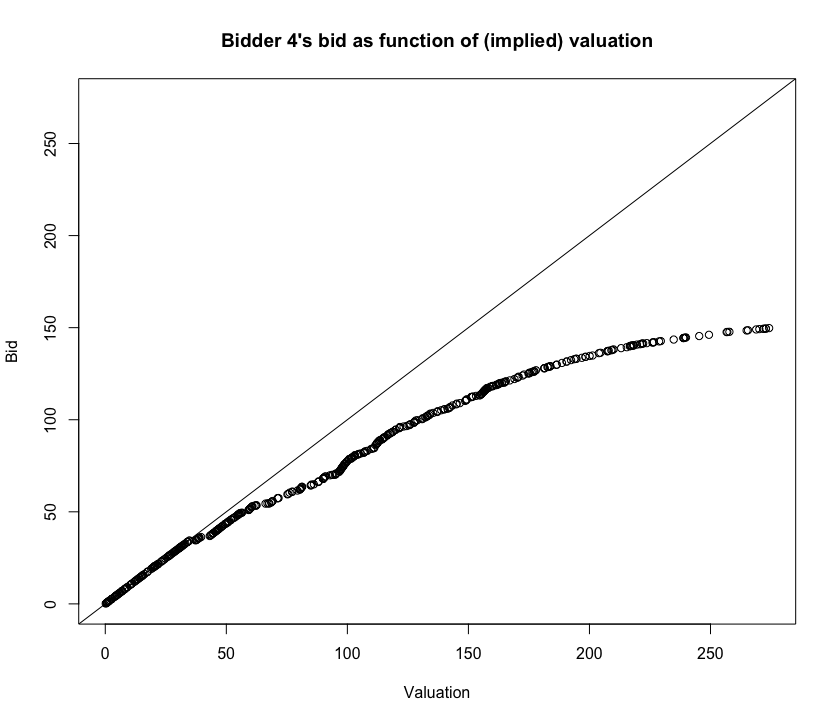
\includegraphics[scale=0.25]{Bid_4.png}
    \end{center}
\end{sol}
\begin{problem}{2}
\end{problem}
\begin{sol}
    I have included the estimated value of $F_U(u_1, u_2, u_3, u_4)$ at all vectors $(u_1, u_2, u_3, u_4)$ where each $u_i$ is either the 25th or 75th percentile of the marginal distribution of $F_U(\cdot)$. I include the estimates in table I:
    \begin{center}
        \begin{table}[!htbp]
            \centering
            \caption{Estimates of $F_U$ at selected vectors}
              \begin{tabular}{lcc}
                  \toprule
                    Quantiles of $u_i$                & $F_U(u_1, u_2, u_3, u_4)      $     & Predicted (under independence)            \\
                  \midrule
                    (0.25, 0.25, 0.25, 0.25) & 0.000 & 0.0039\\
                    (0.75, 0.25, 0.25, 0.25) & 0.018 & 0.0117\\
                    (0.25, 0.75, 0.25, 0.25) & 0.006 & 0.0117\\
                    (0.75, 0.75, 0.25, 0.25) & 0.046 & 0.0352\\
                    (0.25, 0.25, 0.75, 0.25) & 0.006 & 0.0117\\
                    (0.75, 0.25, 0.75, 0.25) & 0.034 & 0.0352\\
                    (0.25, 0.75, 0.75, 0.25) & 0.030 & 0.0352\\
                    (0.75, 0.75, 0.75, 0.25) & 0.102 & 0.1055\\
                    (0.25, 0.25, 0.25, 0.75) & 0.006 & 0.0117\\
                    (0.75, 0.25, 0.25, 0.75) & 0.050 & 0.0352\\
                    (0.25, 0.75, 0.25, 0.75) & 0.028 & 0.0352\\
                    (0.75, 0.75, 0.25, 0.75) & 0.124 & 0.1055\\
                    (0.25, 0.25, 0.75, 0.75) & 0.022 & 0.0352\\
                    (0.75, 0.25, 0.75, 0.75) & 0.098 & 0.1055\\
                    (0.25, 0.75, 0.75, 0.75) & 0.092 & 0.1055\\
                    (0.75, 0.75, 0.75, 0.75) & 0.304 & 0.3164\\
                  \bottomrule
              \end{tabular}
            \label{tab:FU_computation}
          \end{table}
    \end{center} 
\end{sol}
\begin{problem}{3}
\end{problem}
\begin{sol}
If bidders were symmetric, we would observe a number of things. First, we would see that the quantiles of the marginal distribution $F_U(\cdot)$ would be the same (or relatively similar) across bidders. In our data, we see that the 25th quantiles for each bidder are $(49.56, 38.24, 43.01, 41.03)$ and the 75th quantiles are $(151.85, 144.43, 145.40, 154.81)$. We can see that while they are overall relatively similar, there is enough variation to suggest that symmetry may not be completely satisfied. Of course, we would need to compare more quantiles to be able to say anything definitive. Furthermore, under symmetry, we would also see that the marginal distributions of implied valuations would be roughly similar. Upon inspection of the graphs included in part 1, we can see that symmetry is not completely satisfied. While bidders 2-4 seem pretty similar, it seems like bidder 1 is a bit different. As such, the assumption of symmetry seems like it isn't totally satisfied.
\end{sol}
\begin{problem}{4}
\end{problem}
\begin{sol}
Under independence, we would observe that $F_U(u_1, u_2, u_3, u_4)$ would be the product of the marginal distributions $F_U(\cdot)$. To test this, we could compare the estimated distribution function $\hat{F}_U$ to the theoretical distribution function under independence. Under the assumption of independence, the joint distribution will be the product of the marginal distributions. As such, for any quantiles $q_1, q_2, q_3, q_4$ of bidders 1, 2, 3, and 4 respectively, independence would require that \[F_U(q_1, q_2, q_3, q_4) = F_U(q_1) F_U(q_2) F_U(q_3) F_U(q_4)\]
In Table I, we see that the empirical cdf is relatively similar to the theoretical cdf under the assumption of independence. While there are some minor deviations, differences between the empirical cdf and the theoretical cdf are to be expected given that we only have 500 observations for each bidder. 

To see this more formally, we may look at the correlation between each bidder's implied valuations. While correlation will not definitively tell us whether valuations are independent, if the correlation is extremely low then it is relatively likely that bidders have independent valuations. I compute the pairwise correlation between each bidder's estimated valuations and include the results in Table II:
\begin{center}
    \begin{table}[!htbp]
        \centering
        \caption{Correlation between valuations}
          \begin{tabular}{lc}
              \toprule
                Bidders               & Cor($u_i$, $u_j$)             \\
              \midrule
                (1,2) & -0.033\\
                (1,3) & -0.002\\
                (1,4)& 0.022\\
                (2,3) & 0.018\\
                (2,4) & 0.001\\
                (3,4) & 0.018\\
              \bottomrule
          \end{tabular}
        \label{tab:Value_cor}
      \end{table}
\end{center} 
The correlation between bidders' expected valuations are all very close to zero, suggesting that independence is likely satisfied. That being said, we have not conducted a formal test and cannot take a definitive stance. 
\end{sol}
\begin{problem}{5}
\end{problem}
\begin{sol}
    We now assume that bidders have independent and symmetric valuations and estimate the marginal density of valuations. We plot the estimated marginal density in the following figure, alongside the marginal densities for each bidder computed in the previous part. In the figure, the thick black line is the estimated marginal density under the assumption of independence and symmetry. The orange, red, blue, and green lines represent the marginal distributions of bidders 1, 2, 3, and 4, respectively.
    \begin{center}
    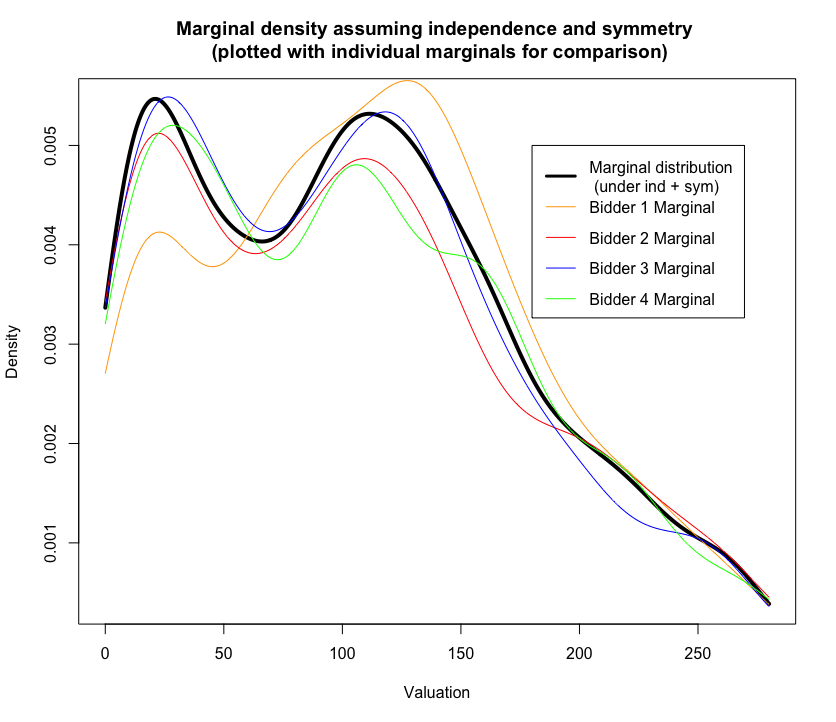
\includegraphics[scale=0.45]{Marginal_plot.png}
    \end{center}
    While the overall shape of the marginal distribution is similar to each of the individual marginal distributions, it doesn't seem to perfectly align with the data. Namely, bidder 1's marginal distribution is significantly different from the estimated distribution. The marginals of bidders 2-4 seem to align more closely with the marginal distribution under symmetry and independence. I

    I also include the cdf of the marginal distribution below, with the individual bidders' valuation cdfs plotted in different colors for comparison. Again, we see that bidders 2-4 appear to be similar, whereas bidder 1 is different.
    \begin{center}
        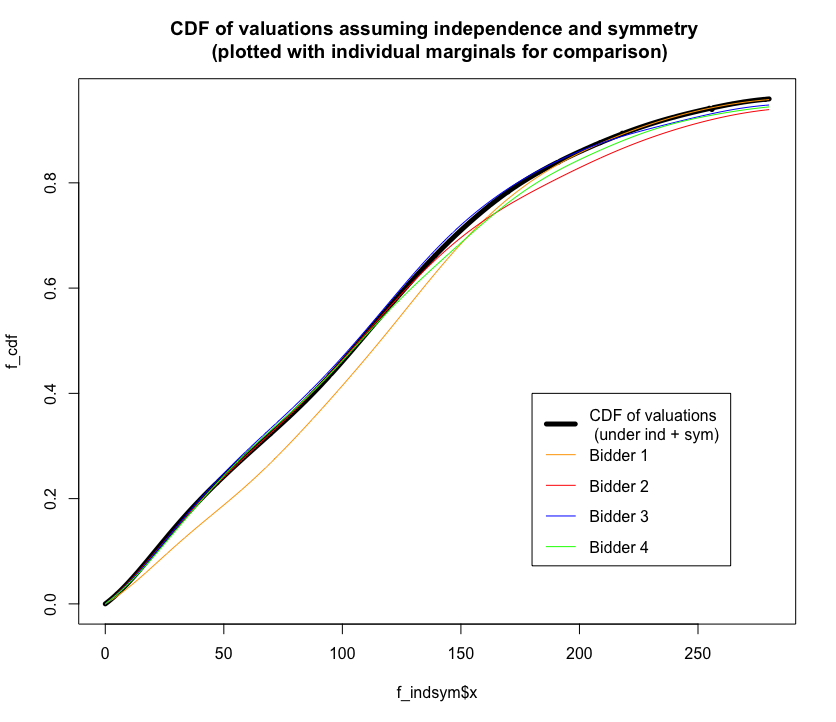
\includegraphics[scale=0.45]{CDF_val.png}
    \end{center}
\end{sol}
\begin{problem}{6}
\end{problem}
\begin{sol}
    I now re-estimate the model by imposing the assumption of symmetric independent private values from the onset. 
\end{sol}


\end{document}